\section{Synchronous Algebras}
\label{sec:synchronous-algebras}

In this section, we introduce and study the ``elementary'' properties of "synchronous algebras".

\subsection{Types \& Dependent Sets}

\paragraph*{Motivation.} The axiomatization of a semigroup reflects the algebraic structure of
finite words: these objects can be concatenated, in an associative way---reflecting the linearity of 
words. Now observe that elements of $\WellFormed$ are still linear, but
not all words can be concatenated together: for instance, $\pair{a}{\pad}$
cannot be followed by $\pair{a}{b}$.
Formally, given two words $u, v \in \WellFormed$, to decide if $uv \in \WellFormed$
it is necessary and sufficient to know if the last pair of $u$ and first pair of $v$
consists of a pair of proper letters (denoted by \AP$\intro*\LL$), a pair of a proper letter and a blank/padding symbol (\AP$\intro*\LB$) or a pair of a blank/padding symbol and a proper letter (\AP$\intro*\BL$). This information is called the \AP""letter-type"" of an element of $\SigmaPair$.

We then define the \AP""type"" of a word of $(\SigmaPair)^+$ as the pair $(\alpha, \beta)$,
usually written $\alpha \to \beta$, of the "letter-types" of its first and last letters.
It is then routine to check that the possible types of "well-formed words" are
\[
	\intro*\types \defeq \big\{
		\LL\to\LL,\; \LL\to\LB,\; \LB\to\LB,\; \LL\to\BL,\; \BL\to\BL
	\big\}.
\]
For the sake of readability, we will write $\alpha$ instead of $\alpha \to \alpha$
for $\alpha \in \{\LL, \LB, \BL\}$.

One non-trivial point lies in the following innocuous question: what is the "type" of the empty word? Any "type" of $\types$ sounds like an acceptable answer. But then
it would be natural to say that the concatenation of $\pair{aaa}{aaa}$ of "type" $\LL$ with the empty word of "type" $\LL\to\LB$ should be $\pair{aaa}{aaa}$ of "type" $\LL\to\LB$. Automata-wise,
this would represent a sequence of transitions $\pair{a}{a}, \pair{a}{a}, \pair{a}{a}$ together with
the promise that the next transition would have a padding symbol on its second tape. But then, 
one has to formalize the idea that the two elements $\pair{aaa}{aaa}$ of type $\LL$ and $\LL\to\LB$
represent the same underlying pair of words of $\Sigma^*\times\Sigma^*$: this idea will be captured by what we call a "dependency relation". A more natural solution would be to simply introduce a
new type for the empty word (or to forbid it), but we show in \Cref{apdx:counterexample} that
the resulting notion of algebras cannot capture the property of being a "$\+V$-relation".

% \paragraph{Synchronous words.}
% \AP Given an alphabet $\Sigma$, let $\AP\intro*\SigmaPair$ denote the alphabet consisting of all pairs
% $\pair{a}{b}$, $\pair{a}{\pad}$ and $\pair{\pad}{a}$ where $a,b$ range over $\Sigma$.
% A word $u \in (\SigmaPair)^+$ is \AP""well-formed"", "aka" \reintro(word){synchronous}, if every letter of the form
% $\pair{a}{\pad}$ (resp.~$\pair{\pad}{a}$), except for the last, is followed by a letters of the 
% form $\pair{b}{\pad}$ (resp.~$\pair{\pad}{b}$), where $a,b \in \Sigma$.
% For instance, the words $\pair{abbab}{aa\pad\pad\pad}$ and $\pair{\pad\pad\pad}{baa}$
% are "well-formed", but neither are $\pair{a\pad b}{b a \pad}$ nor $\pair{a\pad b}{a a a}$.

% The \AP ""letter-type"" of a letter in $\SigmaPair$ is defined to be
% $\LL$ if the letter is of the form $\pair{a}{b}$, $\LB$ if it of the form $\pair{a}{\pad}$,
% and $\BL$ if it is of the form $\pair{\pad}{a}$, where $a,b \in \Sigma$---note that $l$ stands
% for ``letter'' and $b$ for ``blank''.
% The \AP ""type"" of a "well-formed" word $u \in (\SigmaPair)^+$ consists of the pair
% $(\alpha,\beta)$, denoted $\alpha\to\beta$, of the "letter-types" of its first letter and its last letter.
% We write $\AP \intro*\typeW{u}{\alpha\to\beta}$ to mean that
% $u$ has "type" $\alpha \to \beta$.
% The types of "well-formed words" are:


% Observe that if $\typeW{u}{\alpha \to \beta}$ and $\typeW{v}{\beta'\to\gamma}$ are "well-formed", 
% then $uv$ is "well-formed" if, and only if, $\beta = \beta'$, or [$\beta = \LL$ and
% $\beta' \in \{\LB, \BL\}$], in which case $uv$ has "type" $\alpha\to\gamma$, and we say
% that the types $\alpha\to\beta$ and $\beta'\to\gamma$ are \AP ""compatible"".
% For instance:
% \[
% 	% \typeW{\pair{aba}{bbb}}{\LL}\cdot
% 	% \typeW{\pair{aab}{a\pad\pad}}{\LL\to\LB} =
% 	% \typeW{\pair{abaaab}{bbba\pad\pad}}{\LL\to\LB}.
% 	% \quad\text{and}\quad
% 	\typeW{\pair{ab}{bb}}{\LL}\cdot
% 	\typeW{\pair{a}{\pad}}{\LB} = 
% 	\typeW{\pair{aba}{bb\pad}}{\LL\to\LB}.
% \]

% \paragraph*{Empty Word.} Note that for now we talked about non-empty words. The empty word is
% quite different from them since it can potentially have any type. Indeed, it makes
% both sense to declare for instance that
% \[
% 	\typeW{\varepsilon}{\LL}\cdot
% 	\typeW{\pair{aba}{bbb}}{\LL}\cdot
% 	\typeW{\varepsilon}{\LL\to\LB}\cdot 
% 	\typeW{\pair{ab}{\pad\pad}}{\LB} =
% 	\typeW{\pair{abaab}{bbb\pad\pad}}{\LL\to\LB}.
% \]
% If one allow all possible "types" for $\varepsilon$, one needs to have
% a way to say that the elements they represent are ``equivalent'' in some sense.

A \AP""$\types$-typed set"" (or \reintro{typed set} for short) consists of
a tuple $\?X = (X_\tau)_{\tau \in \types}$, where each $X_\tau$ is a set.
Instead of $x \in X_\tau$, we will often write \AP$\intro*\type{x}{\tau} \in \?X$.
A \AP""map between typed sets"" $\?X$ and $\?Y$ is a collection of functions
$X_\tau \to Y_\tau$ for each "type" $\tau$.
Similarly, a subset of $\?X$ is a tuple of subsets of $X_\tau$ for each "type" $\tau$.
To make the notations less heavy, we will often think of
"typed sets" as sets with type annotations rather than tuples, and ask that
all operators/constructions should preserve this "type".

\begin{definition}
	\label{def:dependency}
	A \AP""dependency relation"" over a "typed set" $\?X$ consists of
	a reflexive and symmetric relation $\intro*\dep$ over
	\AP$\intro*\disunion \?X \defeq \bigcup_{\tau \in \types} X_\tau \times \{\tau\}$,
	such that for all $\type{x}{\sigma}, \type{y}{\sigma} \in \?X$,
	if $\type{x}{\sigma} \dep \type{y}{\sigma}$,
	then $\type{x}{\sigma} = \type{y}{\tau}$.

	Crucially, we do not ask for "this relation@dependency" to be transitive---in some examples the "dependency relation" will be an equivalence relation, but not always (\Cref{ex:last_letter_is_a_if_big_diff}), and
	this non-transitivity is actually an important feature, motivated amongst other by the
	"syntactic congruence" and \Cref{coro:syntactic-congruence-is-syntactic-dependency}.

	A \AP""dependent set"" is a "$\types$-typed set" together with a
	"dependency relation" over it. A \AP""closed subset"" of a "dependent set" $\langle \?X, \dep \rangle$ is a subset $C \subseteq \?X$ such that for all
	$x, x' \in \?X$, if $x \dep x'$ then $x \in C \iff x' \in C$.\footnote{In other
	words, $C$ is a union of equivalence classes of the transitive closure of $\dep$.}
\end{definition}
\begin{figure}[htb]
	\begin{center}
		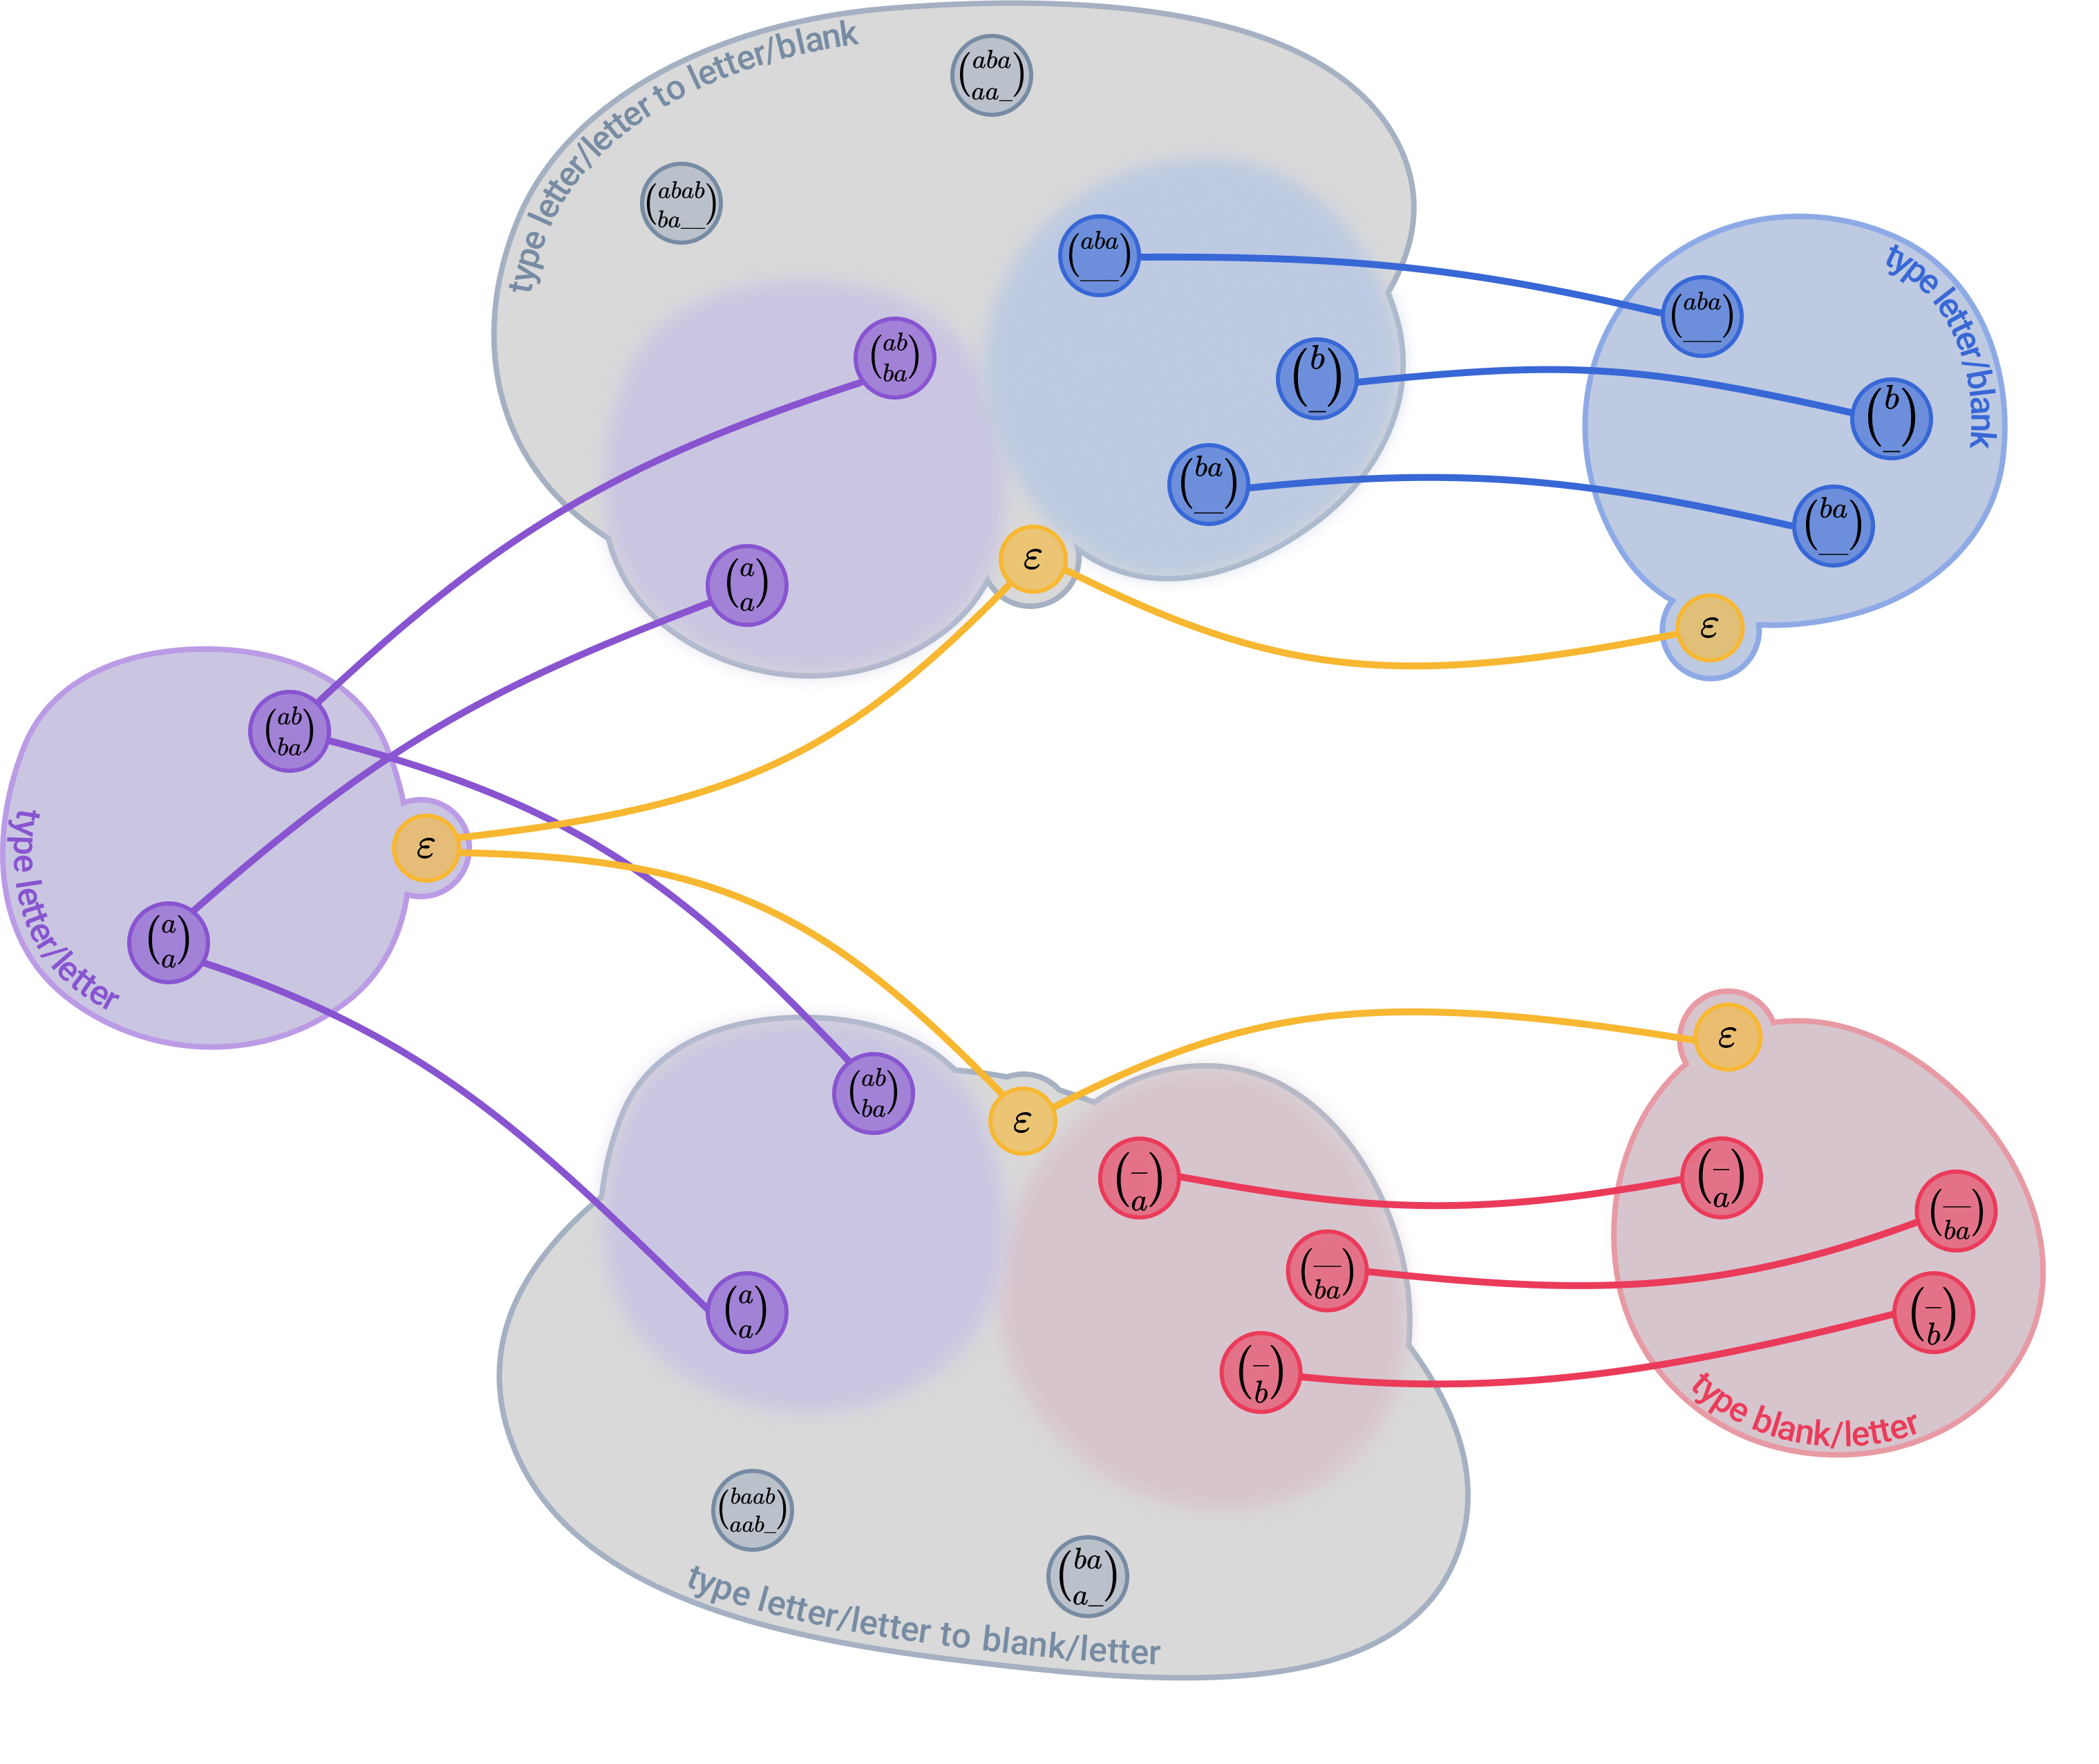
\includegraphics[width=\linewidth]{fig/algebra/free_algebras.png}
	\end{center}
	\caption{
		\label{fig:free_algebras}
		Representation of the "dependent set" $\Sync\Sigma$ of "synchronous words".
		Coloured edges represent the "dependency relation", and self-loops are not drawn. 
	} 
\end{figure}
\begin{example}
	Given a finite alphabet $\Sigma$, let $\intro*\Sync{\Sigma}$ be\footnote{The index refers to the arity of the relations we are considering: here we focus on binary relations, but all constructions can be generalized to higher arities.} the "dependent set" of ""synchronous words"" defined by:
	\vspace{-1.25em}
	\begin{multicols}{2}
	\begin{itemize}
		\item $(\Sync{\Sigma})_{\LL} \defeq (\Sigma\times \Sigma)^*$,
		\item $(\Sync{\Sigma})_{\LL\to\LB} \defeq (\Sigma\times \Sigma)^*(\Sigma\times \pad)^*$,
		\item $(\Sync{\Sigma})_{\LB} \defeq (\Sigma\times \pad)^*$,
		\columnbreak
		\vfill
		\item $(\Sync{\Sigma})_{\LL\to\BL} \defeq (\Sigma\times \Sigma)^*(\pad\times \Sigma)^*$,
		\item $(\Sync{\Sigma})_{\BL} \defeq (\pad\times \Sigma)^*$.
	\end{itemize}
	\end{multicols}
	\vspace{-1em}
	Moreover, $\dep$ is the reflexive and symmetric closure of the relation that
	identifies $\type{u}{\LL}$ with $\type{u}{\LL\to\beta}$ for all
	$u \in (\Sigma\times\Sigma^*)$ and $\beta \in \{\LB,\BL\}$, 
	and $\type{u}{\LL\to\LB}$ with $\type{u}{\LB}$
	for $u \in (\Sigma\times\pad)^*$,
	and $\type{u}{\LL\to\BL}$ with $\type{u}{\BL}$
	for $u \in (\pad\times\Sigma)^*$.
	This structure is depicted in \Cref{fig:free_algebras}.
\end{example}

% Given a set $X$, the \AP""dependent set induced by a set"" $X$ is defined as
% having a copy of $X$ for every "type", and moreover, $\type{x}{\sigma} \dep \type{x}{\tau}$
% for all $x \in X$ and all "types" $\sigma, \tau$.

Given a "relation" $\+R \subseteq \Sigma^* \times \Sigma^*$, we denote by
$\AP\intro*\proj{\+R} = \{\type{(u,v)}{\tau} \mid \type{(u,v)}{\tau} \in \Sync{\Sigma} \text{ and } (u,v) \in \+R\}$
the "closed subset" of $\Sync{\Sigma}$ induced by $\+R$.

\begin{fact}
	The map $\+R \mapsto \proj{\+R}$ is a bijection between
	"relations" and "closed subsets" of $\Sync{\Sigma}$.
\end{fact}

\begin{proof}
	Let $f$ be the function which maps a closed subset $C$ of $\Sync{\Sigma}$ to
	$\{(u,v) \in \Sigma^* \times \Sigma^* \mid \type{(u,v)}{\tau} \in C \text{ for some $\tau \in \types$} \}$. It then follows that $f\circ \proj{-}$ (resp.~$\proj{f(-)}$) is the identity
	on subsets of $\Sigma^* \times \Sigma^*$ (resp.~"closed subsets" of $\Sync{\Sigma}$).
\end{proof}

\subsection{Synchronous Algebras}

One key property of "types" is that some of them can be concatenated to produce other types.
We say that two types $\sigma, \tau \in \types$ are \AP""compatible""
when there exists non-empty words $u,v \in \WellFormed$ of "type" $\sigma$
and $\tau$, respectively, such that $uv$ is "well-formed".
Said otherwise, $\alpha \to \beta$ is "compatible" with $\beta' \to \gamma$
if either $\beta = \beta'$ or $\beta = \LL$---indeed, for this last case
note that "eg" the concatenation of $\pair{aaa}{aaa}$ of type $\LL$ with
$\pair{\pad\pad}{aa}$ of type $\BL$ is "well-formed".
Lastly, if $\alpha\to \beta$ is "compatible with" $\beta'\to\gamma$,
we define their product as \AP $(\alpha\to\beta)\intro*\concattype(\beta'\to\gamma) \defeq \alpha \to \gamma$.
Note that this partial operation is associative, in the following sense: for $\rho,\sigma,\tau \in \types$, $(\rho\concattype\sigma) \concattype \tau$ is well-defined if and only if
$\rho\concattype(\sigma\concattype \tau)$ is well-defined, in which case both "types" are equal.
This implies that the notion of "compatibility" of types can be unambiguously
lifted to finite lists of "types" $\tau_1,\hdots,\tau_n$.

\begin{definition}
	\label{def:synchronous-algebra}
	A \AP""synchronous algebra"" $\langle \?A, \cdot, \dep \rangle$ consists of a "dependent set" $\langle \?A, \dep \rangle$ together
	with a partial binary operation $\cdot$ on $\?A$, called \AP""product"" such that:
	\begin{itemize}
		\item for $\type{x}{\sigma}, \type{y}{\tau} \in \?A$,
			$\type{x}{\sigma} \cdot \type{y}{\tau}$ is defined "iff" $\sigma$ and $\tau$
			are "compatible",
		\item \emph{associativity:} for all $\type{x}{\rho}, \type{y}{\sigma}, \type{z}{\tau} \in \?A$, if $\rho, \sigma, \tau$ are "compatible":
		\[
			(\type{x}{\rho} \cdot \type{y}{\sigma}) \cdot \type{z}{\tau} 
			= \type{x}{\rho} \cdot (\type{y}{\sigma} \cdot \type{z}{\tau}),
		\]
		\item \emph{``monotonicity'':} for all $\type{x}{\sigma}, \type{x'}{\sigma'}, \type{y}{\tau} \in \?A$, if $\type{x}{\sigma} \dep \type{x'}{\sigma'}$ and
		both $\sigma,\tau$ and $\sigma', \tau$ are "compatible", then
		$\type{x}{\sigma}\cdot \type{y}{\tau} \dep \type{x'}{\sigma'}\cdot \type{y}{\tau}$,
		and dually if $\tau,\sigma$ and $\tau, \sigma'$ are "compatible", then 
		$\type{y}{\tau}\cdot \type{x}{\sigma} \dep \type{y}{\tau}\cdot \type{x'}{\sigma'}$,
		\item \emph{units:} for each type $\tau$ there is an element $\type{1}{\tau} \in \?A$ 
			such that for any $\type{x}{\sigma} \in \?A$, then
			$\type{1}{\tau} \cdot \type{x}{\sigma} \dep \type{x}{\sigma}$
			if $\tau$ and $\sigma$ are "compatible",
			and $\type{x}{\sigma} \cdot \type{1}{\tau} \dep \type{x}{\sigma}$
			if $\sigma$ and $\tau$ are "compatible",
			and moreover, $\type{1}{\LL\to\beta} = \type{1}{\LL}\cdot \type{1}{\beta}$
			for $\beta \in \{\LB,\BL\}$.
	\end{itemize}
\end{definition}

Note in particular that for any type $\tau \in \{\LL,\LB,\BL\}$,
then $\type{1}{\tau} \cdot \type{x}{\tau} \dep \type{x}{\tau}$
but since $\type{1}{\tau} \cdot \type{x}{\tau}$ has "type" $\tau$ and $\dep$ is a
"dependency relation", then $\type{1}{\tau} \cdot \type{x}{\tau} = \type{x}{\tau}$.
This implies in particular that restricting $\langle \?A, \cdot \rangle$
to a type $\LL$, $\LB$ or $\BL$ yields a monoid.
These are called the three \AP""underlying monoids"" of $\?A$.
The canonical example of "synchronous algebras" is "synchronous words" $\Sync\Sigma$ under 
concatenation. Its "underlying monoids" are $(\Sigma\times\Sigma)^*$,
$(\Sigma\times\{\pad\})^*$ and $(\{\pad\}\times\Sigma)^*$.

\begin{fact}
	\label{fact:closed-subset-units}
	Any "closed subset" of $\?A$ either contains all units, or none of them.
\end{fact}

\begin{proof}
	From $\type{1}{\LL \to \LB} = \type{1}{\LL}\cdot \type{1}{\LB}$ we have
	$\type{1}{\LL} \dep \type{1}{\LL \to \LB}$
	and $\type{1}{\LL \to \LB} \dep \type{1}{\LB}$.
	By symmetry between $\LB$ and $\BL$, we also have
	$\type{1}{\LL} \dep \type{1}{\LL\to\BL}$ and $\type{1}{\LL\to\BL} \dep \type{1}{\BL}$.
	Hence, if a "closed subset" of $\?A$ contains at least one unit, then it must contain them all.
\end{proof}

Note that the "product" induces a monoid left (resp.~right) action of the
"underlying monoid" $\?A_{\LL}$ (resp.~$\?A_{\LB}$) on the set $\?A_{\LL\to\LB}$.
Moreover, $\type{x}{\LL} \mapsto \type{x}{\LL} \cdot \type{1}{\LB}$
identifies any element of "type" $\LL$ with an element of "type" $\LL\to\LB$.
Over $\Sync{\Sigma}$, these identifications are injective, but it need not be the
case in general. Note also that in general,
$\type{x}{\LL} \cdot \type{1}{\LL\to\LB} = \type{x}{\LL} \cdot \type{1}{\LL}
\cdot \type{1}{\LB} = \type{x}{\LL} \cdot \type{1}{\LB}$.

\begin{remark}
	There exists a monad over the category of "dependent sets" whose
	"Eilenberg-Moore algebras" exactly correspond to
	"synchronous algebras", see \Cref{apdx:monads}.
\end{remark}

\AP""Morphisms of synchronous algebras"" are defined naturally as
maps that preserve the "type", units, the "product" and the "dependency relation".

\paragraph*{Free algebras}
$\Sync\Sigma$ is free in the sense that
for any "synchronous algebra" $\?A$, there is a natural bijection between
"synchronous algebra morphisms" $\Sync\Sigma \to \?A$
and "maps of typed sets" $\SigmaPair \to \?A$.
Said otherwise, "synchronous algebra morphisms" are uniquely defined by
their value on $\SigmaPair$.

\subsection{Recognizability}

Given a "synchronous algebra" $\?A$, a "morphism@@sync" $\phi\colon \Sync{\Sigma} \to \?A$
and a "closed subset" $\Acc \subseteq \?A$ called ``accepting set'',
we say that $\langle \phi, \?A, \Acc \rangle$
\AP""recognizes@@sync"" a relation $\+R \subseteq \Sigma^* \times \Sigma^*$
when $\proj{\+R} = \phi^{-1}[\Acc]$.
We extend the notion of "recognizability@@sync" to $\langle \phi, \?A\rangle$
or to simply $\?A$ by existential quantification over the missing elements in the tuple $\langle \phi, \?A, \Acc \rangle$.

\paragraph*{Synchronous algebra induced by a monoid}
A monoid morphism $\phi\colon (\SigmaPair)^* \to M$
naturally ""induces@@sync"" a "synchronous algebra morphism"
\AP$\intro*\inducedmor{\phi} \colon \Sync\Sigma \to \intro*\inducedalg{M}$,
where:
\begin{itemize}
	\item $\inducedalg{M}$ has for every "type" $\tau$ a copy of $M$,
	and $\dep$ is $\{(\type{x}{\sigma}, \type{x}{\tau}) \mid x \in M, \sigma, \tau \in \types\}$,
	\item for all $\type{x}{\sigma}, \type{y}{\tau} \in \inducedalg{M}$
	with "compatible type", $\type{x}{\sigma} \cdot \type{y}{\tau} \defeq \type{(x\cdot y)}{\sigma\concattype\tau}$,
	\item $\inducedmor{\phi}\pair{a}{b} \defeq \type{\bigl(\phi\pair{a}{b}\bigr)}{\LL}$,
		$\inducedmor{\phi}\pair{a}{\pad} \defeq \type{\bigl(\phi\pair{a}{\pad}\bigr)}{\LB}$,
		and $\inducedmor{\phi}\pair{\pad}{a} \defeq \type{\bigl(\phi\pair{\pad}{a}\bigr)}{\BL}$.
\end{itemize}
The algebra simply duplicates $M$ as many times as needed and identifies
two elements together when they originated from the same element of $M$.
\begin{fact}
	\label{fact:induced-morphism}
	If $\phi$ recognizes $\+R$ for some "relation" $\+R \subseteq \Sigma^* \times \Sigma^*$ seen as a language over $\SigmaPair$, then $\inducedmor{\phi}$ "recognizes@@sync" $\+R$.
\end{fact}

\paragraph*{Consolidation of a synchronous algebra}
Given a "synchronous algebra morphism" $\phi\colon \Sync\Sigma \to \?A$,
define its \AP""consolidation""\footnote{Named by analogy with Tilson's construction \cite[\S 3, p.~102]{tilson_categories_1987}.} as the semigroup morphism
$\intro*\consol{\phi}\colon (\SigmaPair)^* \to \reintro*\consol{\?A}$, where
$\consol{\?A}$ is the monoid obtained from
$\disunion{\?A}$ by first merging units,
by adding a zero (denoted by $0$), and extending $\cdot$
to be a total function by letting all missing products equal $0$,
and $\consol{\phi}$ sends a word $u \in (\SigmaPair)^*$ to%
\vspace{-1.25em}
\begin{multicols}{2}%
	\begin{itemize}%
		\item $0$ if $u$ is not "well-formed",
		\item $\phi(\type{u}{\LL})$ if $u \in (\Sigma\times \Sigma)^*$,
		\item $\phi(\type{u}{\LB})$ if $u \in (\Sigma\times \pad)^+$,
		\item $\phi(\type{u}{\BL})$ if $u \in (\pad\times \Sigma)^+$,
		\item $\phi(\type{u}{\LL\to\LB})$ if $u \in (\Sigma\times \Sigma)^+(\Sigma\times \pad)^+$,
		\item $\phi(\type{u}{\LL\to\BL})$ if $u \in (\Sigma\times \Sigma)^+(\pad\times \Sigma)^+$.
	\end{itemize}
\end{multicols}
\vspace{-1.25em}
Note that this operation disregards the "dependency relation" of $\?A$.
\begin{fact}
	\label{fact:consolidation}
	If $\phi$ "recognizes@@sync" some "relation" $\proj{\+R}$,
	then $\consol{\phi}$ recognizes $\+R$, when seen as
	a language over $\SigmaPair$.
\end{fact}

The following result follows from \Cref{fact:induced-morphism,fact:consolidation,fact:synchronous-is-regular}.
\begin{proposition}
	\label{prop:synchronous-iff-finite}
	A "relation" is "synchronous" if and only if it is "recognized@@sync"
	by a finite "synchronous algebra".
\end{proposition}

Let us continue with a slightly less trivial example of "algebra@synchronous algebra".

% \begin{example}
% 	Given $p,q,r \in \Np$, let $\?Z_{p,q,r}$ be the "synchronous algebra" defined by:
% 	\begin{itemize}
% 		\item its "underlying monoids" of "type" $\LL$,
% 			$\LB$ and $\BL$ are
% 			$\Z/p\Z$, $\Z/q\Z$ and $\Z/r\Z$ under addition, respectively.
% 		\item $(\?Z_{p,q,r})_{\LL\to\LB} = \Z/p\Z \times \Z/q\Z$ and \\
% 			$(\?Z_{p,q,r})_{\LL\to\BL} = \Z/p\Z \times \Z/r\Z$,
% 			with natural addition
% 		\item the units are the zeroes,
% 		\item $\dep$ identifies $\bar x \in \Z/p\Z$ with
% 		$(\bar x, \bar 0) \in \Z/p\Z \times \Z/q\Z$
% 		and with $(\bar x, \bar 0) \in \Z/p\Z \times \Z/r\Z$,
% 		\item similarly, it identifies $\bar x \in \Z/q\Z$ with
% 		$(\bar 0, \bar x) \in \Z/p\Z \times \Z/q\Z$
% 		and dually, it identifies  $\bar x \in \Z/r\Z$ 
% 		with $(\bar 0, \bar x) \in \Z/p\Z \times \Z/r\Z$.
% 	\end{itemize}
% 	This "algebra@@sync" "recognizes@@sync" recognizes "eg"
% 	\begin{align*}
% 		\bigl\{
% 			(a^n, a^m) \in a^*\times a^* \;\big\vert\;
% 			\min(n,m) \dep 1 &
% 			\!\!\mod{p} \text{,\; and } \bigr.\\
% 			\quad n-m \dep 2 &
% 			\!\!\mod{q} \text{ if $n > m$} \text{,\; and } \\
% 			\quad \bigl. 3(m-n) \dep -1 &
% 			\!\!\mod{r} \text{ if $m > n$}
% 				\hphantom{\text{,\; and }}
% 		\bigr\}
% 	\end{align*}
% 	via the "morphism@@sync" defined by 
% 	\[
% 		\phi\pair{a}{a} \defeq \type{1}{\LL},\quad
% 		\phi\pair{a}{\pad} \defeq \type{1}{\LB},\quad\text{and}\quad
% 		\phi\pair{\pad}{a} \defeq \type{3}{\LB}.
% 	\]
% 	\todo{Small figure of a word and evaluation of some subwords over it.}
% \end{example}
\begin{example}[Group relations: {\Cref{ex:group-languages}, cont'd.}]
	\label{ex:algebra-Zpq}
	Fix $p,q \in \N_{>0}$. Let $\?Z_{p,q}$ denote the algebra whose "underlying monoids" are:
	\begin{itemize}
		\item the trivial monoid $(0,+)$ for "type" $\LL$,
		\item the cyclic monoid $(\Z/p\Z,+)$ for "type" $\LB$,
		\item the cyclic monoid $(\Z/q\Z,+)$ for "type" $\BL$.
	\end{itemize}
	Moreover, the sets $Z_{\LL\to\LB}$ and $Z_{\LL\to\BL}$ are defined
	as $\Z/p\Z$ and $\Z/q\Z$, respectively.
	The product is addition---we identify $\type{0}{\LL}$ with the zero of $\Z/p\Z$ and
	of $\Z/q\Z$. We denote by $\bar k$ the equivalence class of $k\in \Z$ in
	$\Z/n\Z$ when $n$ is clear from context.
	The "dependency relation" identifies (1) all units together and (2) $\type{x}{\sigma}$ with $\type{1}{\tau} \cdot \type{x}{\sigma}$ and $\type{x}{\sigma} \cdot \type{1}{\tau}$ when the "types" are "compatible".
	
	Let $\phi\colon \Sync\Sigma \to \?Z_{p,q}$ be the "synchronous algebra morphism"
	defined by
	\[
		\phi \pair{a}{b} \defeq  \type{\bar 0}{\LL}, 
		\quad
		\phi \pair{a}{\pad} \defeq \type{\bar 1}{\LB},
		\quad
		\phi \pair{\pad}{a} \defeq \type{\bar 1}{\BL}
		\quad\text{and}\quad
		\phi(\type{\varepsilon}{\tau}) \defeq \type{\bar 0}{\tau}
		\text{ for $\tau \in \types$}.
	\]
	This "morphism@@sync" recognizes any "relation" of the form 
	\begin{align*}
		\+R^{I,J} \defeq \big\{
			(u,v) \;\big\vert\; & |u| > |v| \text{ and } (|u| - |v| \bmod{p}) \in I, \text{ or} \\
			& |u| < |v| \text{ and } (|v| - |u| \bmod{q}) \in J.
		\hphantom{\text{ or}}\big\},
	\end{align*}
	where $I \subseteq \Z/p\Z$ and $J \subseteq \Z/q\Z$ are such that $\bar 0 \not\in I$
	and $\bar 0 \not\in J$. This last condition is necessary because the accepting set
	has to be a "closed subset" of $\?Z_{p,q}$: if $\bar 0$ was in $I$, then we would need
	$\bar 0 \in J$, but also to add $\type{\bar 0}{\LL}$ to the accepting set: this would "recognize@@sync"
	\begin{align*}
		\big\{
			(u,v) \;\big\vert\; & |u| > |v| \text{ and } (|u| - |v| \bmod{p}) \in I, \text{ or} \\
			& |u| < |v| \text{ and } (|v| - |u| \bmod{q}) \in J, \text{ or } |u| = |v| \big\}.
	\end{align*}
	Note also that all "relations" $\+R^{I,J}$ with $\bar 0 \not\in I$
	and $\bar 0 \not\in J$ are "group relations": letting $G$ be the group $\Z/p\Z \times \Z/q\Z$,
	$\+R$ can be written as $\WellFormed\cap \psi^{-1}[I \times \{0\} \cup \{0\} \times J]$ where $\psi \colon (\SigmaPair)^* \to G$ is the monoid morphism defined by $\psi\pair{a}{b} \defeq 
	(\bar 0, \bar 0)$, $\psi\pair{a}{\pad} \defeq (\bar 1, \bar 0)$ and $\psi\pair{\pad}{a} \defeq
	(\bar 0, \bar 1)$.
\end{example}


\subsection{Syntactic Morphisms \& Algebras}
\label{sec:syntactic-morphism}

\AP\phantomintro{\SyntSAM}\phantomintro{\SyntSA}\phantomintro{syntactic synchronous algebra morphism}\phantomintro{syntactic synchronous algebra}\phantomintro(sync){Syntactic morphism theorem}
\vspace{-2em}
\begin{restatable}[\reintro(sync){Syntactic morphism theorem}]{lemma}{syntacticmorphismtheorem}
	\label{lem:syntactic-morphism-theorem}
	For each relation $\+R$, there exists a surjective "synchronous algebra morphism"
	\[\reintro*\SyntSAM{\+R}\colon \Sync{\Sigma} \surj \reintro*\SyntSA{\+R}\]
	that "recognizes@@sync" $\+R$ and is such that for any other
	surjective "synchronous algebra morphism"
	$\phi\colon \Sync{\Sigma} \surj \?B$
	"recognizing@@sync" $\+R$, there exists a
	"synchronous algebra morphism" $\psi \colon \?B \surj \SyntSA{\+R}$
	such that the diagram
	\begin{center}
		\begin{tikzcd}[ampersand replacement=\&]
			\Sync{\Sigma} 
				\arrow[twoheadrightarrow]{r}{\SyntSAM{\+R}}
				\arrow[twoheadrightarrow, swap]{dr}{\phi}
			\& \SyntSA{\+R} \\
			\& \?B, \arrow[twoheadrightarrow, swap]{u}{\psi}
		\end{tikzcd}
	\end{center}
	commutes.
	The objects $\SyntSAM{\+R}$ and $\SyntSA{\+R}$ are called the \reintro{syntactic synchronous algebra morphism}
	and \reintro{syntactic synchronous algebra} of $\+R$, respectively.
	Moreover, these objects are unique up to "isomorphisms" of the "algebra@@sync".
\end{restatable}

\begin{corollary}[of \Cref{prop:synchronous-iff-finite,lem:syntactic-morphism-theorem}]
	A "relation" is "synchronous" if and only if its "syntactic synchronous algebra"
	is finite.
\end{corollary}

The proof of \Cref{lem:syntactic-morphism-theorem}---see \Cref{apdx-proof:lem:syntactic-morphism-theorem}---relies,
as in the case of monoids, on the notion of congruence.

Given a "synchronous algebra" $\langle \?A, \dep, \cdot \rangle$,
a \AP""congruence@@sync"" is any reflexive, symmetric relation $\asympbar$ over $\?A$ which is
coarser than $\dep$, and which is \AP""locally transitive"",
meaning that for all $\type{x}{\sigma}, \type{x'}{\sigma},
\type{y}{\tau}, \type{y'}{\tau} \in \?X$,
if $\type{x'}{\sigma} \asympbar \type{x}{\sigma}$,
$\type{x}{\sigma} \asympbar \type{y}{\tau}$ and
$\type{y}{\tau} \asympbar \type{y'}{\tau}$,
then $\type{x'}{\sigma} \asympbar \type{y'}{\tau}$.\footnote{In particular, it implies that
$\asympbar$ is transitive when restricted to elements of the same type.}

The \AP""quotient structure"" $\intro*\quotient{\?A}{\asympbar}$
of $\?A$ by a "congruence@@sync" $\asympbar$ is defined as follows:
\begin{itemize}
	\item its underlying "typed set" consists of the
		equivalence classes of $\?A$ under the equivalence relation
		$\{(\type{x}{\sigma}, \type{y}{\sigma}) \mid \type{x}{\sigma} \asympbar \type{y}{\sigma}\}$,
		such a class being abusively denoted by \AP$\intro*\equivclass{x}{\asympbar}$,
	\item its "product" is the "product" induced by $\?A$, in the sense
		that $\equivclass{x}{\asympbar}\cdot \equivclass{y}{\asympbar} \defeq \equivclass{xy}{\asympbar}$, and
	\item its "dependency relation" is the relation induced by $\asympbar$,
		"ie" $\equivclass{x}{\asympbar}\dep \equivclass{y}{\asympbar}$ whenever $x \asympbar y$,
	\item its units are defined as the equivalence classes of the units of $\?A$.
\end{itemize}
Moreover, $x \mapsto \equivclass{x}{\asympbar}$ defines a surjective
"morphism of synchronous algebras" from $\?A$ to $\quotient{\?A}{\asympbar}$.

Given a "synchronous algebra" $\langle \?A, \dep, \cdot \rangle$
and a "closed subset" $C \subseteq \?A$, 
we define a "congruence@@sync" \AP$\intro*\congr{C}$, called
\AP""syntactic congruence"" of $C$ over $\?A$ by letting
$\type{a}{\sigma} \congr{C} \type{b}{\tau}$ when for all $x, y \in \?A$
\begin{itemize}
	\item if both
		$x \type{a}{\sigma} y$
		and $x \type{b}{\tau} y$ are defined,
		then $x \type{a}{\sigma} y \in C$
		"iff" $x \type{b}{\tau} y \in C$, and
	\item if both
		$x \type{a}{\sigma}$
		and $x \type{b}{\tau}$ are defined,
		then $x \type{a}{\sigma} \in C$
		"iff" $x \type{b}{\tau} \in C$, and
	\item if both $\type{a}{\sigma} y$
		and $\type{b}{\tau} y$ are defined,
		then $\type{a}{\sigma} y \in C$
		"iff" $\type{b}{\tau} y \in C$.
\end{itemize}
% \footnote{Starting from now, we will sometimes 
% omit the "type" of \emph{some} elements. When this happens, we do not
% make any assumption on the hidden types.}
It is routine to check that the "syntactic congruence" is indeed a "congruence@@sync".
For instance, to prove that $\congr{C}$ is coarser than $\dep$, observe that
if $\type{a}{\sigma} \dep \type{b}{\tau}$, then
for all $x, y$ "st" both $x \type{a}{\sigma} y$
and $x \type{b}{\tau} y$ are defined, then $x \type{a}{\sigma} y \dep x \type{b}{\tau} y$,
and since $C$ is a "closed subset" of $\?A$, $x \type{a}{\sigma} y \in C$ "iff"
$x \type{b}{\tau} y \in C$. The other two conditions are proven in the same fashion.
Note however that while the relation is "locally transitive", it is not
transitive in general.

When $\+R \subseteq \Sigma^* \times\Sigma^*$ is a "relation", we abuse
the notation and write $\congr{\+R}$ to denote
the "syntactic congruence" $\congr{\proj{\+R}}$ of $\proj{\+R}$
in $\Sync\Sigma$.
The existence of the "syntactic morphism@@sync" then follows from
the next proposition, proven in \Cref{apdx-proof:lem:syntactic-morphism-theorem}.

\begin{restatable}{proposition}{propquotientbysyntacticcongruenceissyntacticalgebra}
	\label{prop:quotient-by-syntactic-congruence-is-syntactic-algebra}
	Let $\phi\colon \Sync\Sigma \surj \?A$ be a surjective "synchronous algebra morphism"
	that "recognizes@@sync" $\+R$, say $\proj{\+R} = \phi^{-1}[\Acc]$
	for some "closed subset" $\Acc \subseteq \?A$, then 
	\begin{center}
		\begin{tabular}{rccc}
			$\quotient{\phi}{\congr{\Acc}}\colon$
			& $\Sync\Sigma$
			& $\surj$
			& $\quotient{\?A}{\congr{\Acc}}$\\
			& $u$
			& $\mapsto$
			& $\equivclass{\phi(u)}{\congr{\Acc}}$
		\end{tabular}		
	\end{center}
	is the "syntactic morphism@@sync" of $\+R$.
\end{restatable}

\begin{corollary}
	\label{coro:syntactic-congruence-is-syntactic-dependency}
	In the "syntactic synchronous algebra" $\SyntSA{\+R}$, the "syntactic
	congruence" $\congr{\Acc}$ and the "dependency relation" $\dep$
	coincide. 
\end{corollary}

\begin{proof}
	By \Cref{prop:quotient-by-syntactic-congruence-is-syntactic-algebra}
	applied to the "syntactic morphism@@sync",
	$x \mapsto \equivclass{x}{\congr{\Acc}}$
	is an isomorphism from $\SyntSA{\+R}$ to $\quotient{\SyntSA{\+R}}{\congr{\Acc}}$.
	Hence, $\equivclass{x}{\congr{\Acc}} \dep \equivclass{y}{\congr{\Acc}}$
	in $\quotient{\SyntSA{\+R}}{\congr{\Acc}}$
	"iff" $x \dep y$ in $\SyntSA{\+R}$, for all $x,y \in \SyntSA{\+R}$.
	But then, the "dependency relation" $\dep$ of
	$\quotient{\SyntSA{\+R}}{\congr{\Acc}}$ is, by definition,
	such that $\equivclass{x}{\congr{\Acc}} \dep \equivclass{y}{\congr{\Acc}}$
	"iff" $x \congr{\Acc} y$.
	Putting both equivalences together, we get that
	$x \congr{\Acc} y$ "iff" $x \dep y$ for all $x,y \in \SyntSA{\+R}$.
\end{proof}

We provide in \Cref{ex:last_letter_is_a_if_big_diff}
a simple example of "syntactic synchronous algebra" whose "dependency relation"
is not an equivalence relation.  

% Moreover, this canonical algebraic representation of $\+R$ is computable.
% \begin{proposition}
% 	There is a polynomial space algorithm computing the "syntactic synchronous algebra"
% 	of a "synchronous relation" from a finite "synchronous automaton" accepting it.
% \end{proposition}

% \subsection{Operations on Synchronous Algebras}
% \label{sec:operations}

\paragraph*{Boolean operations}
\AP Given two "synchronous algebras" $\?A$ and $\?B$, define their \emph{Cartesian product}
$\?A \times \?B$ by taking, for each type $\tau$, the Cartesian product $A_\tau \times B_\tau$. 
Units, "product" are defined naturally, and the "dependency relation" is defined
by taking the conjunction over each component.
Then $\negrel \+R$ is "recognized@@sync" by $\?A$, and
$\+R \cup \+S$ and $\+R \cap \+S$ are "recognized@@sync" by $\?A \times \?B$. 

% \begin{fact}
% 	Let $\?A$ and $\?B$ be two "synchronous algebras", "recognizing@@sync"
% 	$\+R$ and $\+S$, respectively.
% 	Then $\negrel \+R$ is "recognized@@sync" by $\?A$, and
% 	$\+R \cup \+S$, $\+R \cap \+S$ and the symmetric difference $\+R \mathop{\Delta} \+S$ are "recognized@@sync" by $\?A \times \?B$. 
% \end{fact}

% \paragraph*{Composition}
% One particularity of relations, compared with languages, is that they can be composed.
% We introduce in \Cref{apdx:sec:composition} an operation on "synchronous algebras" that simulates this operation.